\chapter[Wstęp ]{Wstęp}
Szybki postęp technologiczny zapoczątkowany w XX wieku umożliwił rozwój nowych dziedziń nauki, między innymi robotyki. Obecnie maszyny mogą zastępować ludzi przy wykonywaniu wielu rozmaitych czynności.
Innowacyjne rozwiązania stwarzają jednak potrzebę opracowania wymagającego środowiska testowego. Jedną z takich inicjatyw, mających na celu wspieranie rozwoju i popularyzację robotyki są rozgrywki
RoboCup. W obrębie przedsięwzięcia wyróżnionych jest kilka lig rozgrywek, różniących się zasadami oraz typem robotów biorących udział w zawodach.
Głównym celem przyświecającym organizatorom jest stworzenie do 2050 roku drużyny robotów zdolnej wygrać z ówczesnymi mistrzami świata.
Liga RoboCup budzi zainteresowanie wielu ludzi na całym świecie, wiele środowisk akademickich prowadzi prace z nią związane.
W Polsce nie została jeszcze stworzona drużyna, która wystartowałaby w tych rozgrywkach.
Rozwiązanie problemu stawia przed uczestnikami wyzwania konstukcyjne oraz algorytmiczne. W niniejszej pracy opisane zostaną właśnie te drugie. Rozwiązany zostanie problem sterowania zawodnikiem,
wyznaczania bezkolizyjnej ścieżki do celu oraz rozwiązywania prostych zachowań niezbędnych podczas rozgrywek.
\section{Zakres pracy}
Niniejsza praca jest niejako kontynuacją działań podjętych podczas realizacji pracy inżynierskiej. Tematyka w niej poruszona dotyczy na wstępie samych rozgrywek Robocup, nastepnie (z uwagi na brak 
rzeczywistych modeli) stworzenia nowego testowego środowiska symulacyjnego oraz przystosowania symulatora. Opracowane zostały nowe modele zawodników, zaimplementowany sterownik umożliwiający: kontrolę
 nad prędkością robota, prowadzenie piłki jak i oddawanie strzału.
 W stosunku do poprzednich prac zdecydowano się także na implementację oraz poddanie testom nowego algorytmu nawigacji. Rozwiązanie to zostało przetestowane w takich samych warunkach 
jak rozwiązanie wcześniejsze.
W pracy zostało także jedno z podejść stosowanych do koordynacji i planowania działań zawodników 
\subsection{Liga Robocup}
\subsection{Planowanie działań drużyny robotów}
\section{Cel pracy}
Celem niniejszej pracy było stworzenie środowiska symulacyjnego, umożliwiającego modelowanie rozgrywki robotów w piłkę nożną oraz 
dającego w przyszłości możliwość testowania różnorodnych rozwiązań sterowania drużyną.
Podczas realizacji postawionego zadania starano się zachować w jak największym stopniu realia rozgrywek \texttt{Robocup}, ze szczególnym uwzględnieniem zasad ligi \emph{Small-size League}.
Z racji, iż wczesniejsze prace prowadzono na symulatorze \emph{Player/Stage/Gazebo} zdecydowano się na dalsze prace na tej platformie.
Zachowano schemat przepływu informacji z pracy inżynierskiej. Został on zamieszczony na rysunku \ref{fig:przeplyw_sterowania}. Stosowany w rozgrywach \emph{Small-size League} został
zamodelowany jako osobna warstwa  aplikacji, komunikująca się bezpośrednio z symulatorem. Osobną warstwę stanowi także część aplikacji odpowiedzialna za sterowanie robotem.
\begin{figure}[H]
\centering
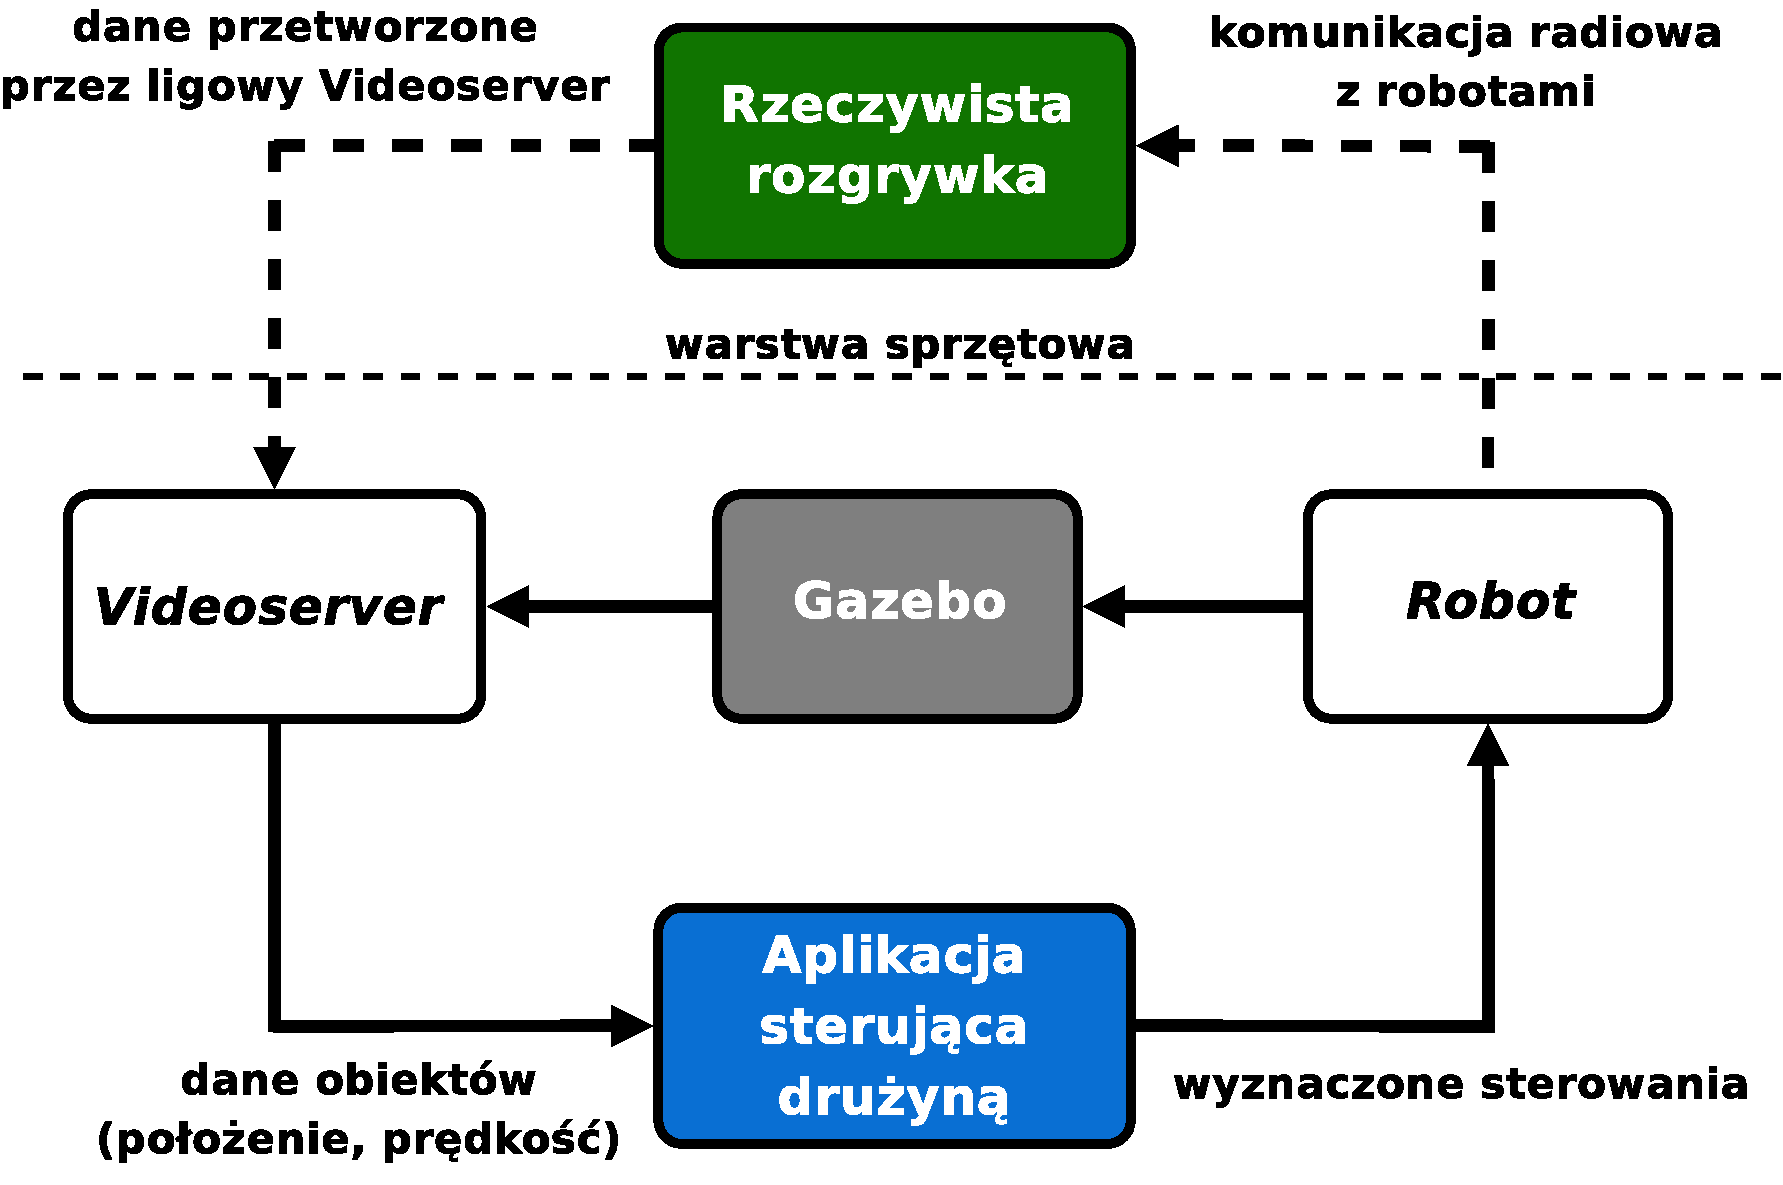
\includegraphics[scale=0.38]{./zalozenia/przeplyw_sterowania.pdf}
\caption{Komunikacja pomiędzy warstwami aplikacji.} \label{fig:przeplyw_sterowania}
\end{figure}
Dzięki takiej architekturze w łatwy sposób można przystosować aplikację do sterowania rzeczywistym robotem pobierającym dane z zewnętrznego serwera.
Zdecydowano się jednak na odejście od modelu robota o napędzie różnicowym. Tego typu baza jezdna wprowadza jednak znaczące ograniczenia na sterowanie takim zawodnikiem. W symulatorze zamodelowane zostały rzeczywiste
roboty biorące udział w rozgrywkach \emph{Small-size League}. Jak już wspomniano w rozdziale \ref{chap:robocup} są to roboty posiadające trzy niezależnie napędzane koła szwedzkie. Sterowanie takim zawodnikiem jest dużo
prostsze. Model został także wyposażony w urządzenie do dryblowania piłki oraz umożliwiające strzał lub podanie.
Przed przystąpieniem do prac nad architekturą aplikacji sterującej dokonano przeglądu rozwiązań stosowanych w rozgrywkach. Ostatecznie zdecydowano się na architekturę 
\mbox{\texttt{STP - Skill Tactics Play}} oryginalny opis można znaleźć w \cite{stp}. Natomiast w niniejszej pracy szerzej została ona omówiona w rozdziale \ref{chap:stp}.

